\section{Digital Output}

In this section you will use the \lstinline|DigitalOutput| sketch.
It is located in the same folder as \lstinline|Blink|, 
to open it go to \lstinline{Examples>00.Hack>DigitalOutput}.
It is exactly the same as the \lstinline|Blink| sketch.
The difference is that you will build two circuits to see how 
the basic digital pins of the Arduino can be used to control electronics
not on the board.

Go ahead and upload it in exactly the same way as you did blink.

You will need the following from the kit:

\setlength{\tabcolsep}{0pt}
\begin{center}
\begin{tabular}{|c| c |}
\hline
    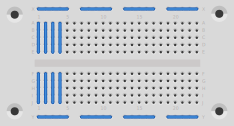
\includegraphics[align=c,width=0.2\textwidth]{./Graphics/breadboard}
    & 
    \begin{minipage}[t]{0.2\textwidth}
        \centering
        1 $\times$ Bread Board 
    \end{minipage}\\ \hline
    \includegraphics[align=c,width=0.2\textwidth]{./Graphics/150_resistor} 
    & 1 $\times$ 150$\Omega$ Resistor \\ \hline
    \includegraphics[align=c,width=0.2\textwidth]{./Graphics/red_led}
    & 1 $\times$ 5mm Red LED \\ \hline
    \includegraphics[align=c,width=0.2\textwidth]{./Graphics/jumper_cables}
    & 2 $\times$ Jumper Cables \\ \hline
  \end{tabular}
\end{center}
%clean this up, maybe even make it into its own thing for hardware.

\subsection{Pin as Source}
First you will use the pin as the source of current that drives the circuit.
This is the easier of the two ways of using the digital pins on an Arduino
to turn things on and off. 

Wire the components listed above as show in the diagram bellow.
You really should disconnect the Arduino from the USB cable,
while the voltages and currents from an Arduino will never be dangerous
touching stray cables with power in them while putting 
\begin{center}
    \includegraphics[width=0.4\textwidth]{./Graphics/PinSource}
\end{center}


\textbf{Note carefully the holes in which the components and wires are plugged in!}
Breadboards will only work if you follow their internal wiring.
In this case two components are connected if they are plugged into the same column
in the middle of the board 
and not separated by the ridge.
For more details on how breadboards work see their section~\ref{subsub:Breadboard}.  

Also note that LEDs only allow current to flow in one direction,
to get the LEDs wired right you need to have one with 
the long leg connected to pin 13
and the short leg connected to the ground (GND) pin.

You should now see both the built in L LED 
and the external red LED blinking in time with each other.

The circuit you build looks like the bellow diagram.
If you are no familiar with circuit diagrams 
and are interested in seeing how it works in detail
see the section on Physics and Hardware.

\begin{center}
\includegraphics[width=0.2\textwidth]{./Graphics/ledOn13.pdf}
\includegraphics[width=0.2\textwidth]{./Graphics/ledOff13.pdf}
\end{center}

As you can see, 
turning pin 13 on connects a source to the circuit 
and current flows.
Turning pin 13 off removes the source from the circuit 
and everything turns off.

\subsection{Pin as Sink}

The circuit in this section uses the same code as the last one,
the difference is that the pin will be used as ground.

\begin{center}
    \includegraphics[width=0.4\textwidth]{./Graphics/PinSink}
\end{center}
Note that even though the circuits look similar they are very different.
The red wire is live and the black is ground.

If you got everything wired up the right way around
you should see the L LED and red external LED blink out of sink 
with each other.

\begin{center}
\includegraphics[width=0.2\textwidth]{./Graphics/ledOn13Rev.pdf}
\includegraphics[width=0.2\textwidth]{./Graphics/ledOff13Rev.pdf}
\end{center}

In the circuit above you see that when pin 13 is on
the voltage it is connected to counteracts the voltage 
from the power pin.
When the pin 13 is off the circuit is closed 
and the external LED turns off.

It is common to use digital pins as both sources
and sinks of current in circuits, which you choose
to use depends on exactly what part you want to
control.


\subsection{Software}
\subsubsection{The Sketch}

\lstinputlisting[style=Arduino]{./Src/blink.src}

This sketch is essentially the same as the \lstinline|Blink| sketch 
you looked at line by line in the last section.

Instead a few words about programming:
It is always good to giver discriptive names to variables so you remember what they refer to.
Naked numbers in the body of a program are generally a bad idea,
especially in long ones,
in the above program you might want to keep the LED on pin 13 high for a second,
since you have just two 500s you need to read the whole program to figure out which one you need to change.

Other than using variables for every number,
something that can get tedious too,
we can use comments to remind you of things you wrote yourself.
Everything between \lstinline|/* */| and after \lstinline|//| is a comment.
This is text ignored by the computer 
and is only used to explain what software does to the people.


\subsubsection{Compiling, Uploading and Executing}

To get a sketch running on the Arduino is it needs to be
translated from human readable text to numbers the computer can understand.
This is done by \textbf{compiling} it. 
Once you have the compiled sketch on your computer it is then
sent by the USB cable to the Arduino which \textbf{executes} it.

At a lower level this is done by the IDE for you,
it first expands the macros we met before into code that makes sense,
runs the GCC cross-compiler for ARV,
and uploads the resulting binary into a predefined place in the memory of the Arduino,
then restarts it.
Once this happens the operating system on the Arduino takes over.
It runs some basic diagnostic tests,
then jumps to the part of memory where setup is located,
runs it,
jumps to where loop is located,
and keeps running that so long as the Arduino has power.

You have already compiled sketches multiple times
by using the upload button.
Using the buttons on the top row of the IDE is the simplest way to
write and edit sketches for the Arduino.

\begin{center}
    \includegraphics[width=0.4\textwidth]{./Graphics/uploading.pdf}
\end{center}

\textbf{Verify:} Compile your sketch without uploading it. Useful for error checking.

\textbf{Upload:} Compile and upload your sketch.
The Arduino begins to execute it immediately.

\textbf{New:} Discard everything you have done and start in a blank sketch.

\textbf{Save:} Save your sketch to the computer.
You should keep in mind that even if you have the sketch uploaded to the Arduino
you can't get back the code from it.
If you want to access a sketch in the future you \textbf{need} to save it.

\textbf{Load:} Open a previously saved sketch.
Again, you can't load a sketch \textit{from} the Arduino,
only sketches that you have saved on your computer.

\textbf{Serial Monitor:} A way for the Arduino to talk back to your computer through the USB cable.
We will see how this works in detail in the Digital Input section.


\subsection{Hardware}
\subsubsection{The Arduino}
\label{subsub:Arduino}

We already talked about what an Arduino is in general,
however looking at the parts which we will be using more closely:

\begin{center}
    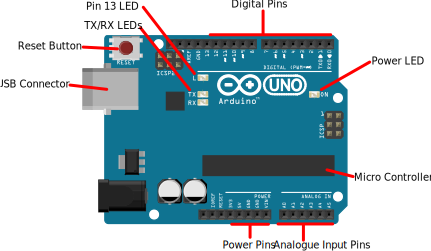
\includegraphics[width=0.4\textwidth]{./Graphics/arduino_label.pdf}
\end{center}

\textbf{Pin 13 LED:} You have already used this extensively, 
the only other thing is that it is used by the Arduino for diagnostic purposes during upload and reboot. 
To you this will look like fast blinking which you didn't tell it to do for about 1 second after either an upload or reboot.

\textbf{TX/RX LED:} These are LEDs that activate when the computers talks to the Arduino (RX),
such as when it uploads a sketch, 
or when the Arduino talks to the computer (TX),
such as when running a serial monitor or connecting through the USB cable.

\textbf{Reset Button:}
This resets the Arduino to the state it had when the program was first uploaded.
This is useful when a sketch you write stops working after something it didn't expect happens.

\textbf{USB Cable:}
The most common way to connect to the Arduino and to give power to it.
Because of the limitations of the USB standard the Arduino is limited to 
5 volts and a few hundred milliamp,
much less than even a AAA battery,
such tiny currents and voltages make it completely safe 
but not able to drive more power hungry components like DC motors directly.

\textbf{Power Pins:}
These are pins which can be used when you need just a simple battery like source,
either in 3 volts or 5 volts.

\textbf{Analogue Input Pins:}
A specialized set of pins that can be used to read continuously varying voltages,
such as light detectors.
Limited to voltages between 0V to 5V.

\textbf{Micro Controller:}
The heart of the Arduino.
All the code lives here.

\textbf{Power LED:}
The first thing you should look at if your Arduino isn't working.

\textbf{Digital Pins:}
A set of pins which can can be used for input or output.
They can only send out and receive high or low signals. 
Pins with a $\sim$ next to the number can approximate an analogue output
by quickly turning on and off see analogue output section.

The advantage of having a micro controller over other arrangements,
such is that Raspberry Pi,
is that it is quite easy to replace the micro controller with another chip
and use it as is in one of your projects.
At between one to three dollars a piece even small hardware projects can have multiple Arduinos embedded within them at a negligible cost and extra power.

\subsubsection{The Bread Board}
\label{subsub:Breadboard}

A breadboard is the circuit equivalent of a Lego set,
and like a Lego set where you put anything has a huge impact on how things get wired.

\begin{center}
    \includegraphics[width=0.4\textwidth]{./Graphics/breadboard_wiring}
\end{center}

The holes in the middle of the board are connected to each other in half columns separated by a ridge in the middle.
On the outside the holes are connected by rows in the same way.
Each blue line above shows which holes are connected together in a circuit.
If you connect a wire to any of them it is as if you had connected it to all of them.

The breadboard you have with the kit is somewhat larger than the one in the diagrams here but is wired on exactly the same principles.

While it isn't as robust as a soldered circuit or printed circuit board 
and making sure that every wire is threaded into the right hole might seem like a pain, 
the flexibly it adds to prototyping makes it more than a worth while trade off.
Every electronic project in the space started off on a breadboard somewhere.


\subsubsection{The Resistor}
Resistors are electrical components which are used to limit the current through, 
or voltage across,
other more sensitive electronic components.
For the circuits which you will be using here they can be considered indestructible.
For an explanation on what current and voltage mean please see the Physics Appendix~\ref{chap:Physics}.


Every resistor is colour coded,
the ones in the kit are 3 band and the following info graphics explains how to read them:
\begin{center}
    \includegraphics[width=0.4\textwidth]{./Graphics/4-Band_Resistor.pdf}
\end{center}

In the above example we have red, purple, green, gold.
This translates to 2, 7, 100,000 $\pm5\%$ which is
$27 \times 100,000 = 2,700,000 \Omega \pm5\%$.
This is a very large resistance, one which you will not be using in any project here.
The resistors you will deal with will be between 10,000$\Omega$ and 100$\Omega$.

At the level of physics a resistor is an anything that follows the rule
$V = IR$ and the equivalent $I = \frac{V}{R}$, $R = \frac{V}{I}$.
Bellow is a current voltage characteristic plot which shows how the current changes in response to changes in voltage for a given idealized resistor.

\begin{center}
    \includegraphics[width=0.4\textwidth]{./Graphics/Resistor_Characteristic}
\end{center}

Unlike LEDs they have no preferred direction and will work equally well whichever way they are plugged in.

In circuits the resistor is most often represented by

\begin{center}
    \includegraphics[width=0.2\textwidth]{./Graphics/resistorSymbol}
\end{center}


\subsubsection{The LED}
LEDs are semiconductor devices,
to understand how they work in detail requires quite involved quantum mechanics,
however to use them successfully in circuits you only need to remember a few simple rules:

\begin{itemize}
\item They will not work bellow a given voltage, 
usually between 1.2-3.4V depending on their colour.
This is called the voltage drop $v_d$.
\item They need a resistor to limit current through them so they do not burnout.
\item During normal operation they will only let current flow in one direction,
if you supply a high enough voltage in the other direction the LED will burnout. 
\end{itemize}

The voltage-current characteristic for an LED,
as you can see there isn't a simple relationship between voltage and current like there is for the resistor.
You will always want to run the LED close to the $v_d$ spot on the diagram.
\begin{center}
    \includegraphics[width=0.4\textwidth]{./Graphics/LED_Characteristic}
\end{center}


Bellow is a diagram on how to wire an LED properly.
It's worth remembering that positive in the direction of the source
and negative in the direction of ground.
\begin{center}
    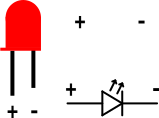
\includegraphics[width=0.4\textwidth]{./Graphics/led_pins}
\end{center}

The last symbol above is how LEDs are most often represented
in diagrams.

